\documentclass[12pt]{scrartcl}
\usepackage{config}
\usepackage{minted}

%\newcommand\mrh{\color{white}\bfseries}
\newcommand\mrc[1]{\begin{tabular}{@{}l@{}} #1 \end{tabular}}
\setlength\arrayrulewidth{0.8pt}

\usemintedstyle{pastie}

\begin{document}
    \hh{Árbol Xor}
    
    
    \vspace{10pt}

    
    \hh{Problema}
    
        Te es dado un entero $N$ y $N - 1$ aristas con pesos. Estas aristas conectan $N$ vértices de tal forma que exista un camino entre cualesquiera dos vértices (es decir, forman un árbol).
        \footnote{Un camino simple en un grafo es definido como una secuencia de $k$ vértices $\{v_1, v_2, \cdots , v_k\}$, tal que para todo $1 \le i \le k - 1$, la arista $\{v_i, v_{i + 1}\}$ existe en el grafo. }
        
        Para cada camino, definimos su peso como el {\bfseries xor} \footnote{or exclusivo, aquí consideramos la operación bit por bit} de cada uno de los pesos de las aristas que componen el camino. Determina la suma de los pesos de todos los caminos simples (no repiten aristas) del árbol \footnote{el camino $\{a, b\}$ se considera el mismo que $\{b, a\}$}.
        
    \hh{Detalles de Implementación}

        Debes implementar la función \textit{Encuentra\_xor()}. Esta función recibe un entero $N$, 3 vectores $u, v$ y $w$, cada uno con $N - 1$ elementos. para cada $0 \le i \le N - 2$, $u[i]$ y $v[i]$ son los vértices que se conectan con la arista $i$, y $w[i]$ es su peso. Esta función debe regresar un entero, la suma de los pesos de todos los caminos.
        La función se vería así:

\begin{minted}{c++}
#include <bits/stdc++.h>
using namespace std;

long long Encuentra_xor(int N, vector<int> u, vector<int> v, vector<int> w) {
    // Implementa esta función.
}
    
\end{minted}

    El evaludor correrá tu programa \textbf{multiples} veces por cada caso.

    \hh{Ejemplos}

               
        {\itshape Ejemplo 1:}
        
        \begin{itemize}
            \item  El evaluador llama la función 
            \begin{center}
                \textit{Encuentra\_xor(5, \{0, 1, 0, 4\}, \{1, 2, 3, 1\}, \{2, 3, 4, 0\})}
            \end{center}
            el árbol en este caso se ilustra en la siguiente imagen:
            
            \begin{center}
                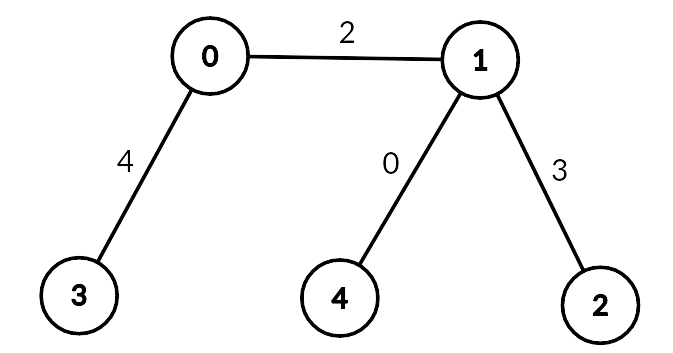
\includegraphics[scale=0.3]{ej1.png}
            \end{center}
            
            \item los xors de los caminos son:

                \begin{center}
                    
                \begin{tabular}{|c||c|c|c|c|c|}
                     \hline
                      $\oplus$ & 0 & 1 & 2 & 3 & 4  \\
                     \hline
                     \hline 
                     0 & 0 & 2 & 1 & 4 & 2 \\
                     \hline 
                     1 & 2 & 0 & 3 & 6 & 0 \\ 
                     \hline
                     2 & 1 & 3 & 0 & 5 & 3 \\
                     \hline
                     3 & 4 & 6 & 5 & 0 & 6 \\
                     \hline
                     4 & 2 & 0 & 3 & 6 & 0 \\
                     \hline
                \end{tabular}
                
                \end{center}
            \item  La función debe regresar 32, la suma del xor de todos los caminos (el camino $\{a, b\}$ se considera el mismo que $\{b, a\}$).
                
        \end{itemize}


        {\itshape Ejemplo 2:}
        \begin{itemize}
            \item El evaluador llama la función 
            \begin{center}
                \textit{Encuentra\_xor(9, \{0, 1, 0, 1, 0, 2, 3, 3\}, \{1, 2, 3, 4, 5, 6, 7, 8\}, \{2, 3, 4, 5, 1, 0, 7, 2\})} 
            \end{center}
            el árbol en este caso es el siguiente:

            \begin{center}
                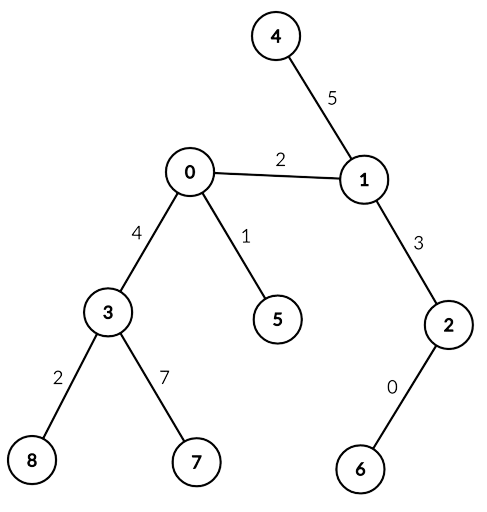
\includegraphics[scale=0.5]{ej2.png}
            \end{center}
            \item La función debe regresar 132.
            
        \end{itemize}
               
        


    
    \hh{Consideraciones}
        \begin{itemize}
            \item $1 \le N \le 2\times10^5$.
            \item Los vectores $u, v$ y $w$ tendrán exactamente $N - 1$ elementos.
            \item Para cada $0 \le i \le N - 2$, se cumple que $0 \le u[i] \neq v[i] < N$. 
            \item Para cada $0 \le i \le N - 2$, se cumple que $0 \le w[i] \le 10^9$.
            \item Se garantiza que el grafo formado por las aristas es un árbol.
            \item Sea $S_N$ la suma total de los valores de $N$ sobre todas las veces que es llamada la función durante un caso. Se garantiza que $S_N \le 2 \times 10^5$.
        \end{itemize}
    
    \hh{Subtareas}


    \begin{itemize}
        \item (10 puntos) $N, S_N \le 2000$.
        \item (20 puntos) Para todo $0 \le i \le N - 2$, se cumple que $w[i] \le 1$.
        \item (25 puntos) Para todo $0 \le i \le N - 2$, se cumple que $u[i] = i, v[i] = i + 1$.
        \item (45 puntos) Sin restricciones adicionales.
    \end{itemize}
\end{document}
